\documentclass[10pt]{beamer}

%packages
\usepackage{babel}
\usepackage[utf8]{inputenc}
\usepackage{amsmath,tabu}
\usepackage{color}
\usepackage{tikz}
\usetikzlibrary{matrix,chains,positioning,decorations.pathreplacing,arrows}
\usetikzlibrary{fit,shapes}
\usetikzlibrary{calc,shadings}
\usepackage{pgfplots}
\usepackage{colortbl}
\usepackage{eurosym}
\usepackage{mathtools}
\usepackage{listings}
\usepackage{tabularx}

\usepackage[style=mla]{biblatex}


%definitions
\usepackage{algorithm,algorithmic}

%theme
\usetheme{Dresden}
\usecolortheme{rose}
\useoutertheme{tree}

%environments
\newenvironment{ExampleGer}{\begin{exampleblock}{Example}}{\end{exampleblock}}

\newenvironment{customlegend}[1][]{%
	\begingroup
	% inits/clears the lists (which might be populated from previous
	% axes):
	\csname pgfplots@init@cleared@structures\endcsname
	\pgfplotsset{#1}%
}{%
	% draws the legend:
	\csname pgfplots@createlegend\endcsname
	\endgroup
}%

%definitions
\def\addlegendimage{\csname pgfplots@addlegendimage\endcsname}
% definition to insert numbers
\pgfkeys{/pgfplots/number in legend/.style={%
		/pgfplots/legend image code/.code={%
			\node at (0.295,-0.0225){#1};
		},%
	},
}

%general
\title{A Simplex based approach to Vertex Enumeration of Arrangements and Polyhedra}
\author{Tilman Hinnerichs}
\institute{Seminar \glqq Selected Topics in Logic and Verification\grqq{} -- TU Dresden}
\date{July 27, 2020}

%presentation
\expandafter\def\expandafter\insertshorttitle\expandafter{%
	\insertshorttitle\hspace{4.5cm}%
	\insertframenumber\,/\,\inserttotalframenumber
}

\definecolor{myblue}{RGB}{80,80,160}
\definecolor{mygreen}{RGB}{80,160,80}
\definecolor{myturk}{RGB}{240,60,60}

\begin{document}
	
\begin{frame}{}
	\titlepage
\end{frame}

\section{The Vertex Enumeration Problem}
\begin{frame}{The paper}
	\textbf{\large{\glqq A Pivoting Algorithm for Convex Hulls and Vertex Enumeration of Arrangements and Polyhedra\grqq{}}}\\
	\vspace{0.5cm}
	Authors: David Avis and Komei Fukuda\\
	Publication year: 1992\\
	Journal: Discrete \& Computational Geometry\\
	\pause 
	\textbf{Cited 751 times} (according to Google Scholar)
	
\end{frame}

\begin{frame}{Outline}
	\setbeamertemplate{section in toc}[sections numbered]
	\tableofcontents
\end{frame}


\begin{frame}{The Vertex Enumeration Problem}
	\begin{definition}[Convex Polyhedron]
		Given a matrix $A=(a_{ij}) \in \mathbb{R}^{m\times n}$ and a vector $b \in \mathbb{R}^m$.\\
		
		A \textit{convex polyhedron} $P$ is defined as
		\begin{equation}
			P = \{ x\in \mathbb{R}^n: Ax+b\geq 0 \}
		\end{equation}
	\end{definition}
	\pause 
	\begin{definition}[Polyhedron Vertex]
		A point $x\in P$ is a \textit{vertex} of $P$ \textbf{iff}\\
		it cannot be written as a convex combination of two other solutions \textbf{iff}\\
		it is the unique solution to a subset of $m$ inequalities solved as equations. 
	\end{definition}
	
\end{frame}

\begin{frame}{The Vertex Enumeration Problem (VEP)}
	\begin{definition}[Vertex Enumeration Problem]
		For a given polytope/polyhedron, hyperplane arrangement $P$ return all vertices of $P$.
		
	\end{definition}
	\pause 
	\begin{alertblock}{Theorem\footnote{Khachiyan et al. [2008]}}
		The VEP is NP-complete.
	\end{alertblock}
	\pause
	Goals:
	\begin{itemize}
		\item should be deterministic
		\item should be fast
		\item shouldn't use too much space
	\end{itemize}
\end{frame}

\begin{frame}{An Example Problem}
	\begin{exampleblock}{Example: Meals for 1 Euro}
	\vspace{0.4cm}
	\begin{tabular}{|p{0.35cm}|l|p{1.5cm}|p{0.9cm}|p{1.cm}|p{0.75cm}|p{1.5cm}|}
		\hline
		Var&Food type&Energy (kcal/100g)&Protein (g)&Calcium (mg)&Price (Euro cents)&Maximum\\
		\hline
		$x_1$&Oatmeal\footnote{Regular LIDL oatmeal}&250&15&40&10&500g\\
		$x_2$&Milk\footnote{Regular Bio LIDL milk}&80&4&130&4&1000g\\
		$x_3$&DD Stollen\footnote{https://fddb.info}&340&7&30&20&200g\\
		\hline
		&\textbf{Min. daily}&\textbf{2000}&\textbf{55}&\textbf{800}&&\\
		\hline
	\end{tabular}
	\vspace{0.4cm}
	\end{exampleblock}	
\end{frame}

\begin{frame}{Putting data into inequalities}
	\begin{exampleblock}{Example: Meals for 1 Euro}
		\begin{equation*}
			A = \begin{bmatrix}
			350&80&340\\
			15&4&7\\
			40&130&30\\
			-10&-4&-20\\
			-1&0&0\\
			0&-1&0\\
			0&0&-1\\
			\end{bmatrix},
			x = \begin{bmatrix}
			x_1\\x_2\\x_3\\
			\end{bmatrix},
			-b = \begin{bmatrix}
			2000\\
			55\\
			800\\
			-100\\
			-5\\
			-10\\
			-2\\
			\end{bmatrix},
			\begin{pmatrix}
			Energy\\
			Protein\\
			Calcium\\
			Price\\
			x_1Max\\
			x_2Max\\
			x_3Max\\
			\end{pmatrix}
		\end{equation*}
	\end{exampleblock}
\end{frame}

\begin{frame}{Polytope visualized}
	\begin{exampleblock}{Example: Meals for 1 Euro}
		\begin{figure}[ht]
			\includegraphics[width = 0.6\textwidth]{allMeals2.png}
			\caption{The exact shape is unknown/expensive}
		\end{figure}
	\end{exampleblock}
\end{frame}

\begin{frame}{An Example Problem}
	\begin{itemize}
		\item Use convex combination to yield infinitely many food combinations
	\end{itemize}
	\pause 
	\begin{definition}[Convex combination]
		A convex combination is a linear combination of points. \\
		
		Let $x_1, x_2, \dots, x_n$ be a finite set of points. A convex combination is a point of the form 
		\begin{equation*}
		y = a_1x_1 + a_2x_2 + \dots + a_nx_n
		\end{equation*}
		while $a_1, \dots, a_n\in\mathbb{R^+}$, and
		\begin{equation*}
		a_1 + \dots + a_n = 1
		\end{equation*}
	\end{definition}
\end{frame}

\section{Approaches to the VEP}
\begin{frame}{Approaches to the VEP}
	\begin{enumerate}
		\item Double-description/Motzkin-based method
		\item Pivot-based methods
		\item Newer methods
	\end{enumerate}
\end{frame}

\section{The \textsc{Simplex} Algorithm}
\begin{frame}{Linear optimization problems}
	\begin{definition}
		Let $ G \subseteq \mathbb{R}^n$ be a polyhedron and $ c \in \mathbb{R}^n$. Then a problem of the form \\
		\vspace{0.15cm}
		\begin{quotation}
			$ z = f(x) = c^T \cdot x \rightarrow min\hspace{1cm} with\ x \in G$
		\end{quotation} 
		is called a \emph{linear} optimization problem.
	\end{definition}
	\pause 
	\begin{exampleblock}{Protein rich meals for 1 Euro}
		We are trying to maximize our protein intake:
		\begin{equation*}
			c =
			\begin{bmatrix}
			15\\4\\7\\
			\end{bmatrix},
			x = \begin{bmatrix}
				x_1\\x_2\\x_3
			\end{bmatrix}
		\end{equation*}
		\begin{equation*}
			z = c^Tx \rightarrow max
		\end{equation*}
	\end{exampleblock}
\end{frame}

\begin{frame}{The \textsc{Simplex} Algorithm}
	\begin{figure}[ht]
		\centering
		\includegraphics[width = 0.2\textwidth]{George_Dantzig.jpg}
		\caption{George Dantzig (1914 - 2005)}
	\end{figure}

	\begin{algorithm}[H]
		\caption{The \textsc{Simplex} Algorithm}
		\label{alg:seq}
		\begin{algorithmic}[1]
			\STATE Find a first feasible vertex
			\STATE Calculate the optimal vertex
		\end{algorithmic}
	\end{algorithm}
\end{frame}

\begin{frame}{From $\geq$ to =}
	The inequalities 
	\begin{equation*}
		Ax + b \geq 0
	\end{equation*}
	describing $P$ are transformed to the equivalent equality system
	\begin{equation*}
		Mx + b = x_p
	\end{equation*}
	with $x\in \mathbb{R}_+^n$, $ x_p \in \mathbb{R}_+^m$, and $M\in \mathbb{R}^{m\times n}$ (if $x\geq 0$)\\
	\pause
	\begin{definition}[Tableau form]
		A linear program of the form \\
		\vspace{0.25cm}
		$ z = f'(x') = c'^T \cdot x' \rightarrow max$ 
		\hspace{0.5cm} with $Mx_N+b=x_B$ with \begin{tabular}{l}
			$x_N:=x,$ \\
			$x_B:=x_p,$\\ $x'\leftrightarrow\begin{pmatrix}
			x_N\\x_B\\
			\end{pmatrix} $\\
			$b\geq 0$
		\end{tabular}  \\
		\vspace{0.15cm}
		is said to be in \textbf{tableau form}.\\
	\end{definition}
\end{frame}

\begin{frame}[fragile]{}
	\begin{exampleblock}{Another example}
	\begin{tabular}{rrrrrrrrrr}
		&$ -z $&$=$& $-30x_1$ &$-$&$45x_2$ &$\rightarrow$& \textbf{$min$}&& \\
		\\
		with&$\cellcolor{cyan}x_3$&$=$&$-4x_1$ &$-$&$3x_2$&$+$&$100$&&\\
		&\cellcolor{cyan}$x_4$&$=$&$-x_1$ & $-$&$2x_2$&$+$&$50$&&\\
		&$x_3,x_4$&,&\cellcolor{orange}$x_1$ &, &\cellcolor{orange}$x_2$&$\geq$&$0$
	\end{tabular} \\
	\vspace{0.5cm}
	\begin{tabular}{ll}
		\cellcolor{orange}\textcolor{orange}{aaa} & non-base variables, with indices $N = \{1,2\}, |N| = n$\\
		\cellcolor{cyan}\textcolor{cyan}{aaa}& base variables, with indices $B = \{3, 4\}, |B| = m$
	\end{tabular}\\

	\vspace{0.5cm}
	\textsc{Simplex}-Tableau: %\hspace{1cm}
	\begingroup
	\def\arraystretch{1.5}
	\begin{tabular}{r|rr|r}
		$ST_0$&$x_1$&$x_2$&$1$\\
		\hline
		$x_3=$&$-4$&$-3$&$100$\\
		$x_4=$&$-1$&$-2$&$50$\\
		\hline
		$-z=$&$-30$&$-45$&$0$
	\end{tabular}
	\endgroup
	\begingroup
	\def\arraystretch{1.5}
	\begin{tabular}{r|r|r}
		$ST_0$&$x_N$&$1$\\
		\hline
		$x_B=$&$M$&$p$\\
		&&\\
		\hline
		$z=$&$q^T$&$q_0$
	\end{tabular}
	\endgroup
	\end{exampleblock}
\end{frame}

\begin{frame}{}
	\begingroup
	\def\arraystretch{1.5}
	\begin{tabular}{r|r|r}
		$ST_0$&$x_N$&$1$\\
		\hline
		$x_B=$&$M$&$p$\\
		\hline
		$z=$&$q^T$&$q_0$
	\end{tabular}
	\endgroup \\
	\vspace{0.25cm}
	$ x_N $ results from $ x $ and $ N $ \\
	$ x_B $ results from  $ x $ and $ B $ \\ 
	$M$ results from $A$ \\
	$p:=b$ \\
	$ q := c' $\\
	$ q_0:=0$ \\
	\vspace{0.25cm}
\end{frame}

\begin{frame}{Visualization of new polytope $P$}
	
	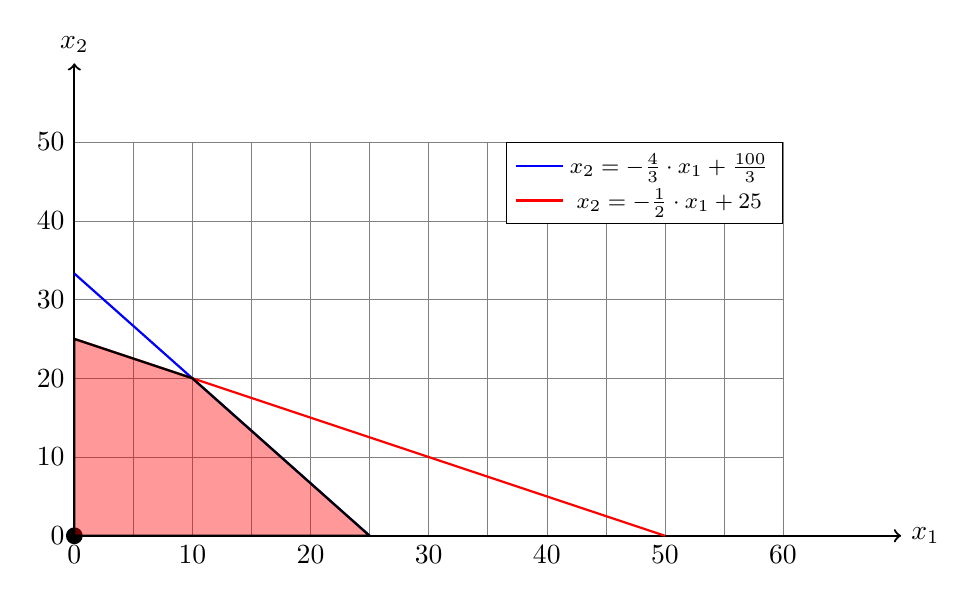
\begin{tikzpicture}[x=0.15cm,y=0.1cm]
	
	\def\xmin{0}
	\def\xmax{60}
	\def\ymin{0}
	\def\ymax{50}
	
	% grid
	\draw[style=help lines, ystep=10, xstep=5] (\xmin,\ymin) grid
	(\xmax,\ymax);
	
	% axes
	\draw[->, thick] (\xmin,\ymin) -- (\xmax+10,\ymin) node[right] {$x_1$};
	\draw[->, thick] (\xmin,\ymin) -- (\xmin,\ymax+10) node[above] {$x_2$};
	
	% xticks and yticks
	\foreach \x in {0,10,...,60}
	\node at (\x, \ymin) [below] {\x};
	\foreach \y in {0,10,...,50}
	\node at (\xmin,\y) [left] {\y};
	
	% plot the data from the file data.dat
	% smooth the curve and mark the data point with a dot
	
	% generate and plot another a curve y = 0.1 x^2 + 2.5
	% this generates the files figure.parabola.gnuplot and figure.parabola.table 
	%\draw[color=red, domain=\xmin:\xmax] plot[id=parabola]
	%function{0.1*x**2 + 2.5} node [right] {$y=0.1\,x^2 + 2.5$};
	\draw [thick, blue](0,33.3) -- (25,0) ;
	\draw [thick, red](0,25) -- (50,0) ;
	
	\node[draw,circle,inner sep=2pt,fill] at (0,0){};
	\filldraw[thick,fill=red,fill opacity=0.4] (0,0) -- (0,25) -- (10,20) -- (25,0) -- (0,0) -- cycle;
	\begin{customlegend}[
	legend entries={ % <= in the following there are the entries
		$ x_2 = -\frac{4}{3}\cdot x_1 + \frac{100}{3} $,
		$x_2 = -\frac{1}{2}\cdot x_1 + 25$
	},
	legend style={at={(60,50)},font=\footnotesize}] % <= to define position and font legend
	% the following are the "images" and numbers in the legend
	\addlegendimage{thick,blue,opacity = 1}
	\addlegendimage{thick,red,opacity = 1}
	\end{customlegend}
	\end{tikzpicture}
\end{frame}

\begin{frame}{Phase 1: Determine first feasible basic solution}
	\begin{algorithm}[H]
		\caption{Phase 1: Determine first feasible basic solution (vertex)}
		\label{alg:seq}
		\begin{algorithmic}[1]
			\IF{trivial solution visible}
			\STATE choose it
			\ENDIF
			\STATE ...
		\end{algorithmic}
	\end{algorithm}
	
	\begin{definition}
		The point \\
		\vspace{0.15cm}
		$x \leftrightarrow \left(\begin{array}{c}  x_B \\ x_N \end{array}\right) = \left(\begin{array}{c}p \\ 0 \end{array}\right)$\\
		\vspace{0.15cm}
		is called \textbf{basic solution}. \\If $p \geq 0$, x is called \textbf{basic feasible solution(BFS)}.
	\end{definition}
\end{frame}

\begin{frame}{Phase 2: Bestimmung der optimalen Ecke}
	\begin{algorithm}[H]
		\caption{Phase 2: Bestimmung der optimalen Ecke}
		\label{alg:seq}
		\begin{algorithmic}[1]
			\WHILE{$\tau\in N$ mit $q_\tau <0$ existiert}
			\STATE Wähle das \textsc{Pivot}-Element $ P_{\sigma \tau} $
			\STATE Berechne mit Hilfe der Tauschungsregeln das neue Simplextableau
			\ENDWHILE
		\end{algorithmic}
	\end{algorithm}
	\pause
	\begin{alertblock}{Satz}
		Das \textsc{Simplex}-Tableau ist optimal gdw. $ p \geq 0 $ und $ q \geq 0 $
	\end{alertblock}
\end{frame}

\begin{frame}{Die Wahl des \textsc{Pivot}-Elements}
	\begingroup
	\def\arraystretch{1.5}
	\begin{tabular}{r|r|r}
		$ST_0$&$x_N$&$1$\\
		\hline
		$x_B=$&$P$&$p$\\
		\hline
		$z=$&$q^T$&$q_0$
	\end{tabular}
	\endgroup
	\\\vspace{0.25cm}
	Wir wählen $\tau\in N$ mit $q_\tau < 0$ beliebig, und bilden daraufhin $ - \dfrac{p_\sigma}{P_{\sigma\tau}} := \min \left\{ -\frac{p_i}{P_{i\tau}} | -\frac{p_i}{P_{i\tau}} < 0, i\in B \right\} $: \\
	\vfill
	
	\begingroup
	\def\arraystretch{1.5}
	\begin{tabular}{r|rr|r}
		$ST_0$&$x_1$&$x_2$&$1$\\
		\hline
		$x_3=$&$-4$&$-3$&$100$\\
		$x_4=$&$-1$&\cellcolor{orange}$-2$&$50$\\
		\hline
		$-z=$&$-30$&$-45$&$0$
	\end{tabular}
	\endgroup
	$\implies \tau := 2, \sigma:=4 $
\end{frame}

\begin{frame}
	\begingroup
	\def\arraystretch{1.5}
	\begin{tabular}{r|rr|r}
		$ST_0$&$x_1$&$x_2$&$1$\\
		\hline
		$x_3=$&$-4$&$-3$&$100$\\
		$x_4=$&$-1$&\cellcolor{orange}$-2$&$50$\\
		\hline
		$-z=$&$-30$&$-45$&$0$
	\end{tabular}\pause\hspace{1cm}
	\def\arraystretch{2}
	\begin{tabular}{r|rr|r}
		$ST_1$&$x_1$&$x_4$&$1$\\
		\hline
		$x_3=$&\only<3->{\cellcolor{orange}}$-\dfrac{5}{2}$&$\dfrac{3}{2}$&$25$\\
		$x_2=$&$-\dfrac{1}{2}$&$-\dfrac{1}{2}$&$25$\\
		\hline
		$-z=$&$-\dfrac{15}{2}$&$\dfrac{45}{2}$&$-1125$
	\end{tabular}
	\\
	\visible<4->{
		\begin{tabular}{r|rr|r}
			$ST_2$&$x_3$&$x_4$&$1$\\
			\hline
			$x_1=$&$-\dfrac{2}{5}$&$\dfrac{3}{5}$&$10$\\
			$x_2=$&$\dfrac{1}{5}$&$-\dfrac{8}{10}$&$20$\\
			\hline
			$-z=$&$3$&$18$&$-1200$
		\end{tabular}
	}
	\endgroup
\end{frame}

\begin{frame}{Properties of the \textsc{Simplex} algorithm}
	
	\begin{itemize}
		\item Does not always terminate
		\begin{itemize}
			\item easily fixable by introducing an ordering among the nodes
		\end{itemize}
	\end{itemize}
	\pause 
	\begin{alertblock}{Theorem}
		For a given basic feasible solution (BFS) $v$ the \textsc{Simplex} algorithm deterministically determines a path from $v$ to the optimal vertex $v*$.
	\end{alertblock}
\end{frame}

\begin{frame}{Some thoughts}
	\begin{enumerate}
		\item What if we choose a pair of indices different from the optimal one in a simplex step?
		\item  
	\end{enumerate}
\end{frame}




\begin{frame}{A visual example}
	
	\begin{exampleblock}{Example: From Avis' lecture notes}
		\begin{equation*}
			A = \begin{bmatrix}
			-1&0&1\\
			0&-1&1\\
			1&0&1\\
			0&1&1\\
			0&0&-1\\
			\end{bmatrix},
			x = \begin{bmatrix}
			x_1\\x_2\\x_3\\
			\end{bmatrix},
			-b = \begin{bmatrix}
			1\\1\\1\\1\\0\\
			\end{bmatrix},
			\begin{tabular}{r}
			$ 1-x_1+x_3\geq 0 $\\
			$ 1-x_2+x_3\geq 0 $\\
			$ 1+x_1+x_3\geq 0 $\\
			$ 1+x_2+x_3\geq 0 $\\
			$ -x_3 \geq 0 $\\
			\end{tabular}
		\end{equation*},
		
		
	\end{exampleblock}
\end{frame}



\begin{frame}{A visual example}
	\begin{example}{Example: From Avis' lecture notes}
		\begin{figure}
			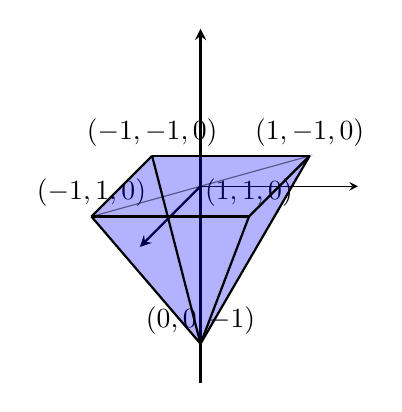
\begin{tikzpicture}
			
			\draw[thick,-stealth] (0,0,0)--(0,0,2); 
			\draw[thick,-stealth] (0,-2.5,0)--(0,2,0);
			\draw[-stealth] (0,0,0)--(2,0,0);
			\coordinate[label={$(0,0,-1)$}] (O) at (0,-2,0);
			\coordinate[label={$(1,1,0)$}] (A1) at (1,0,1);
			\coordinate[label={$(1,-1,0)$}] (A2) at (1,0,-1);
			\coordinate[label={$(-1,1,0)$}] (A3) at (-1,0,1);
			\coordinate[label={$(-1,-1,0)$}] (A4) at (-1,0,-1);
			
			\draw[fill=blue,opacity=0.3] (A1)--(A2)--(A3);
			\draw[fill=blue,opacity=0.3] (A4)--(A2)--(A3);
			\draw[fill=blue,opacity=0.3] (A1)--(O)--(A3);
			\draw[fill=blue,opacity=0.3] (A1)--(O)--(A2);
			\draw[thick](A1)--(A3);
			\draw[thick](A1)--(A2);
			\draw[thick](A4)--(A3);
			\draw[thick](A2)--(A4);
			\draw[thick](O)--(A3);
			\draw[thick](O)--(A1);
			\draw[thick](O)--(A2);
			\draw[thick](O)--(A4);
			\end{tikzpicture}
			\caption{$P$ is a regular pyramid}
		\end{figure}
	\end{example}
\end{frame}

\begin{frame}{The \textsc{Simplex} Algorithm}
	\begin{example}{A linear OP example}
		content...
	\end{example}
\end{frame}

\begin{frame}{Sources}
	\footnotesize
	\begin{thebibliography}{9}
		\bibitem{VEPhard} 
			L. Khachiyan, E. Boros, K. Borys, K. Elbassioni, and V. Gurvich. Generating all verticesof a polyhedron is hard.Discrete and Computational Geometry, 39(1):174–190, 2008.
		
	\end{thebibliography}
\end{frame}

\end{document}